% Created by tikzDevice version 0.12.3.1 on 2021-07-01 16:56:49
% !TEX encoding = UTF-8 Unicode
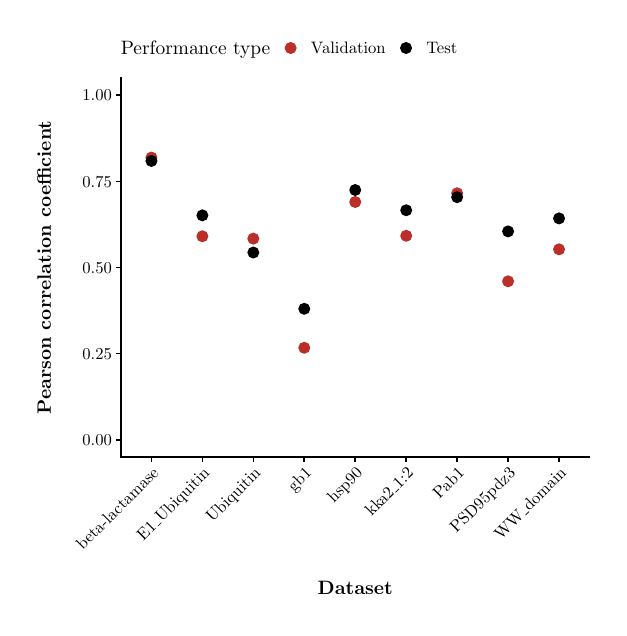
\begin{tikzpicture}[x=1pt,y=1pt]
\definecolor{fillColor}{RGB}{255,255,255}
\path[use as bounding box,fill=fillColor,fill opacity=0.00] (0,0) rectangle (206.56,209.59);
\begin{scope}
\path[clip] ( 33.67, 54.47) rectangle (203.06,191.39);
\definecolor{drawColor}{RGB}{187,46,41}
\definecolor{fillColor}{RGB}{187,46,41}

\path[draw=drawColor,line width= 0.4pt,line join=round,line cap=round,fill=fillColor] ( 63.13,134.21) circle (  1.96);
\definecolor{drawColor}{RGB}{0,0,0}
\definecolor{fillColor}{RGB}{0,0,0}

\path[draw=drawColor,line width= 0.4pt,line join=round,line cap=round,fill=fillColor] ( 63.13,141.77) circle (  1.96);
\definecolor{drawColor}{RGB}{187,46,41}
\definecolor{fillColor}{RGB}{187,46,41}

\path[draw=drawColor,line width= 0.4pt,line join=round,line cap=round,fill=fillColor] (173.60,117.94) circle (  1.96);
\definecolor{drawColor}{RGB}{0,0,0}
\definecolor{fillColor}{RGB}{0,0,0}

\path[draw=drawColor,line width= 0.4pt,line join=round,line cap=round,fill=fillColor] (173.60,135.97) circle (  1.96);
\definecolor{drawColor}{RGB}{187,46,41}
\definecolor{fillColor}{RGB}{187,46,41}

\path[draw=drawColor,line width= 0.4pt,line join=round,line cap=round,fill=fillColor] (155.19,149.76) circle (  1.96);
\definecolor{drawColor}{RGB}{0,0,0}
\definecolor{fillColor}{RGB}{0,0,0}

\path[draw=drawColor,line width= 0.4pt,line join=round,line cap=round,fill=fillColor] (155.19,148.34) circle (  1.96);
\definecolor{drawColor}{RGB}{187,46,41}
\definecolor{fillColor}{RGB}{187,46,41}

\path[draw=drawColor,line width= 0.4pt,line join=round,line cap=round,fill=fillColor] ( 81.54,133.36) circle (  1.96);
\definecolor{drawColor}{RGB}{0,0,0}
\definecolor{fillColor}{RGB}{0,0,0}

\path[draw=drawColor,line width= 0.4pt,line join=round,line cap=round,fill=fillColor] ( 81.54,128.34) circle (  1.96);
\definecolor{drawColor}{RGB}{187,46,41}
\definecolor{fillColor}{RGB}{187,46,41}

\path[draw=drawColor,line width= 0.4pt,line join=round,line cap=round,fill=fillColor] (192.01,129.50) circle (  1.96);
\definecolor{drawColor}{RGB}{0,0,0}
\definecolor{fillColor}{RGB}{0,0,0}

\path[draw=drawColor,line width= 0.4pt,line join=round,line cap=round,fill=fillColor] (192.01,140.67) circle (  1.96);
\definecolor{drawColor}{RGB}{187,46,41}
\definecolor{fillColor}{RGB}{187,46,41}

\path[draw=drawColor,line width= 0.4pt,line join=round,line cap=round,fill=fillColor] ( 44.72,162.66) circle (  1.96);
\definecolor{drawColor}{RGB}{0,0,0}
\definecolor{fillColor}{RGB}{0,0,0}

\path[draw=drawColor,line width= 0.4pt,line join=round,line cap=round,fill=fillColor] ( 44.72,161.43) circle (  1.96);
\definecolor{drawColor}{RGB}{187,46,41}
\definecolor{fillColor}{RGB}{187,46,41}

\path[draw=drawColor,line width= 0.4pt,line join=round,line cap=round,fill=fillColor] ( 99.95, 93.91) circle (  1.96);
\definecolor{drawColor}{RGB}{0,0,0}
\definecolor{fillColor}{RGB}{0,0,0}

\path[draw=drawColor,line width= 0.4pt,line join=round,line cap=round,fill=fillColor] ( 99.95,108.00) circle (  1.96);
\definecolor{drawColor}{RGB}{187,46,41}
\definecolor{fillColor}{RGB}{187,46,41}

\path[draw=drawColor,line width= 0.4pt,line join=round,line cap=round,fill=fillColor] (118.36,146.60) circle (  1.96);
\definecolor{drawColor}{RGB}{0,0,0}
\definecolor{fillColor}{RGB}{0,0,0}

\path[draw=drawColor,line width= 0.4pt,line join=round,line cap=round,fill=fillColor] (118.36,150.93) circle (  1.96);
\definecolor{drawColor}{RGB}{187,46,41}
\definecolor{fillColor}{RGB}{187,46,41}

\path[draw=drawColor,line width= 0.4pt,line join=round,line cap=round,fill=fillColor] (136.78,134.38) circle (  1.96);
\definecolor{drawColor}{RGB}{0,0,0}
\definecolor{fillColor}{RGB}{0,0,0}

\path[draw=drawColor,line width= 0.4pt,line join=round,line cap=round,fill=fillColor] (136.78,143.61) circle (  1.96);
\end{scope}
\begin{scope}
\path[clip] (  0.00,  0.00) rectangle (206.56,209.59);
\definecolor{drawColor}{RGB}{0,0,0}

\path[draw=drawColor,line width= 0.6pt,line join=round,line cap=rect] ( 33.67, 54.47) --
	( 33.67,191.39);
\end{scope}
\begin{scope}
\path[clip] (  0.00,  0.00) rectangle (206.56,209.59);
\definecolor{drawColor}{RGB}{0,0,0}

\node[text=drawColor,anchor=base east,inner sep=0pt, outer sep=0pt, scale=  0.60] at ( 30.42, 58.63) {0.00};

\node[text=drawColor,anchor=base east,inner sep=0pt, outer sep=0pt, scale=  0.60] at ( 30.42, 89.74) {0.25};

\node[text=drawColor,anchor=base east,inner sep=0pt, outer sep=0pt, scale=  0.60] at ( 30.42,120.86) {0.50};

\node[text=drawColor,anchor=base east,inner sep=0pt, outer sep=0pt, scale=  0.60] at ( 30.42,151.98) {0.75};

\node[text=drawColor,anchor=base east,inner sep=0pt, outer sep=0pt, scale=  0.60] at ( 30.42,183.10) {1.00};
\end{scope}
\begin{scope}
\path[clip] (  0.00,  0.00) rectangle (206.56,209.59);
\definecolor{drawColor}{RGB}{0,0,0}

\path[draw=drawColor,line width= 0.6pt,line join=round] ( 31.92, 60.69) --
	( 33.67, 60.69);

\path[draw=drawColor,line width= 0.6pt,line join=round] ( 31.92, 91.81) --
	( 33.67, 91.81);

\path[draw=drawColor,line width= 0.6pt,line join=round] ( 31.92,122.93) --
	( 33.67,122.93);

\path[draw=drawColor,line width= 0.6pt,line join=round] ( 31.92,154.05) --
	( 33.67,154.05);

\path[draw=drawColor,line width= 0.6pt,line join=round] ( 31.92,185.16) --
	( 33.67,185.16);
\end{scope}
\begin{scope}
\path[clip] (  0.00,  0.00) rectangle (206.56,209.59);
\definecolor{drawColor}{RGB}{0,0,0}

\path[draw=drawColor,line width= 0.6pt,line join=round,line cap=rect] ( 33.67, 54.47) --
	(203.06, 54.47);
\end{scope}
\begin{scope}
\path[clip] (  0.00,  0.00) rectangle (206.56,209.59);
\definecolor{drawColor}{RGB}{0,0,0}

\path[draw=drawColor,line width= 0.6pt,line join=round] ( 44.72, 52.72) --
	( 44.72, 54.47);

\path[draw=drawColor,line width= 0.6pt,line join=round] ( 63.13, 52.72) --
	( 63.13, 54.47);

\path[draw=drawColor,line width= 0.6pt,line join=round] ( 81.54, 52.72) --
	( 81.54, 54.47);

\path[draw=drawColor,line width= 0.6pt,line join=round] ( 99.95, 52.72) --
	( 99.95, 54.47);

\path[draw=drawColor,line width= 0.6pt,line join=round] (118.36, 52.72) --
	(118.36, 54.47);

\path[draw=drawColor,line width= 0.6pt,line join=round] (136.78, 52.72) --
	(136.78, 54.47);

\path[draw=drawColor,line width= 0.6pt,line join=round] (155.19, 52.72) --
	(155.19, 54.47);

\path[draw=drawColor,line width= 0.6pt,line join=round] (173.60, 52.72) --
	(173.60, 54.47);

\path[draw=drawColor,line width= 0.6pt,line join=round] (192.01, 52.72) --
	(192.01, 54.47);
\end{scope}
\begin{scope}
\path[clip] (  0.00,  0.00) rectangle (206.56,209.59);
\definecolor{drawColor}{RGB}{0,0,0}

\node[text=drawColor,rotate= 45.00,anchor=base east,inner sep=0pt, outer sep=0pt, scale=  0.60] at ( 47.64, 48.30) {beta-lactamase};

\node[text=drawColor,rotate= 45.00,anchor=base east,inner sep=0pt, outer sep=0pt, scale=  0.60] at ( 66.05, 48.30) {E1\_Ubiquitin};

\node[text=drawColor,rotate= 45.00,anchor=base east,inner sep=0pt, outer sep=0pt, scale=  0.60] at ( 84.46, 48.30) {Ubiquitin};

\node[text=drawColor,rotate= 45.00,anchor=base east,inner sep=0pt, outer sep=0pt, scale=  0.60] at (102.88, 48.30) {gb1};

\node[text=drawColor,rotate= 45.00,anchor=base east,inner sep=0pt, outer sep=0pt, scale=  0.60] at (121.29, 48.30) {hsp90};

\node[text=drawColor,rotate= 45.00,anchor=base east,inner sep=0pt, outer sep=0pt, scale=  0.60] at (139.70, 48.30) {kka2\_1:2};

\node[text=drawColor,rotate= 45.00,anchor=base east,inner sep=0pt, outer sep=0pt, scale=  0.60] at (158.11, 48.30) {Pab1};

\node[text=drawColor,rotate= 45.00,anchor=base east,inner sep=0pt, outer sep=0pt, scale=  0.60] at (176.52, 48.30) {PSD95pdz3};

\node[text=drawColor,rotate= 45.00,anchor=base east,inner sep=0pt, outer sep=0pt, scale=  0.60] at (194.93, 48.30) {WW\_domain};
\end{scope}
\begin{scope}
\path[clip] (  0.00,  0.00) rectangle (206.56,209.59);
\definecolor{drawColor}{RGB}{0,0,0}

\node[text=drawColor,anchor=base,inner sep=0pt, outer sep=0pt, scale=  0.70] at (118.36,  4.86) {\bfseries Dataset};
\end{scope}
\begin{scope}
\path[clip] (  0.00,  0.00) rectangle (206.56,209.59);
\definecolor{drawColor}{RGB}{0,0,0}

\node[text=drawColor,rotate= 90.00,anchor=base,inner sep=0pt, outer sep=0pt, scale=  0.70] at (  8.39,122.93) {\bfseries Pearson correlation coefficient};
\end{scope}
\begin{scope}
\path[clip] (  0.00,  0.00) rectangle (206.56,209.59);
\definecolor{drawColor}{RGB}{0,0,0}

\node[text=drawColor,anchor=base west,inner sep=0pt, outer sep=0pt, scale=  0.70] at ( 33.67,199.82) {Performance type};
\end{scope}
\begin{scope}
\path[clip] (  0.00,  0.00) rectangle (206.56,209.59);
\definecolor{drawColor}{RGB}{187,46,41}
\definecolor{fillColor}{RGB}{187,46,41}

\path[draw=drawColor,line width= 0.4pt,line join=round,line cap=round,fill=fillColor] ( 95.02,202.24) circle (  1.96);
\end{scope}
\begin{scope}
\path[clip] (  0.00,  0.00) rectangle (206.56,209.59);
\definecolor{drawColor}{RGB}{0,0,0}
\definecolor{fillColor}{RGB}{0,0,0}

\path[draw=drawColor,line width= 0.4pt,line join=round,line cap=round,fill=fillColor] (136.72,202.24) circle (  1.96);
\end{scope}
\begin{scope}
\path[clip] (  0.00,  0.00) rectangle (206.56,209.59);
\definecolor{drawColor}{RGB}{0,0,0}

\node[text=drawColor,anchor=base west,inner sep=0pt, outer sep=0pt, scale=  0.60] at (102.37,200.17) {Validation};
\end{scope}
\begin{scope}
\path[clip] (  0.00,  0.00) rectangle (206.56,209.59);
\definecolor{drawColor}{RGB}{0,0,0}

\node[text=drawColor,anchor=base west,inner sep=0pt, outer sep=0pt, scale=  0.60] at (144.07,200.17) {Test};
\end{scope}
\end{tikzpicture}
